% !TEX encoding = UTF-8 Unicode

\chapter{Ortografia}

\section{Alfabeto}

\begin{table}[ht]
    \centering
    \begin{tabular}{lr}
        \toprule
        Scritto     &   Letto \\
        \midrule
        sh          &   \textbf{sci}operare (italiano)\\
        dh          &   \textbf{th}e (inglese) \\
        zh          &   gara\textbf{ge} (francese)\\
        xh          &   \textbf{j}ack (inglese) \\
        gj          &   \textbf{g}ianduia (italiano)\\
        j           &   i (italiano)\\
        q           &   \textbf{c}iao (italiano)\\
        k           &   \textbf{c}asa (italiano)\\ 
        y           &   D\textbf{u} domain (francese)\\
        z           &   ro\textbf{s}a (italiano) \\
        ç           &   \textbf{c}isterna (italiano) \\
        c           &   \textbf{z}ona (italiano) \\
        g           &   \textbf{g}ola \\
        \bottomrule
    \end{tabular}
\end{table}


\begin{figure}[ht]
    \centering
    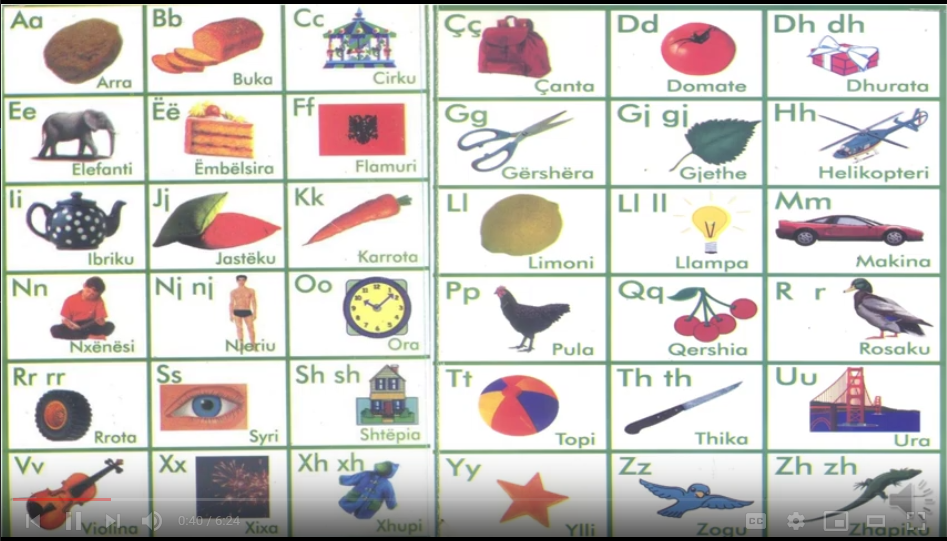
\includegraphics[width=0.8\textwidth]{src/images/alfabetoAlbanese.PNG}
    \caption{Alfabeto albanese}
\end{figure}

\chapter{L'essenziale nella comunicazione base}

\section{Saluti}

\begin{table}[ht]
    \centering
    \begin{tabular}{lr}
        \toprule
        Italiano    &   Albanese \\
        \midrule
        \addTranslationRow{Buon Mattino}\\
        \addTranslationRow{Buon pomeriggio}\\
        \addTranslationRow{Buona sera}\\
        \addTranslationRow{Buona notte}\\
        \addTranslationRow{A presto}\\
        \addTranslationRow{Piacere}\\
        \addTranslationRow{Ci vediamo presto}\\
        \addTranslationRow{Arrivederci}\\
        \addTranslationRow{Addio}\\
        \addTranslationRow{Ciao}\\
        \addTranslationRow{Bene}\\
        \bottomrule
    \end{tabular}
\end{table}

\section{Espressioni comuni}

\begin{table}[ht]
    \centering
    \begin{tabular}{lr}
        \toprule
        Italiano    &   Albanese \\
        \midrule
        \addTranslationRow{Grazie}\\
        \addTranslationRow{Per favore}\\
        \addTranslationRow{Perdonami}\\
        \addTranslationRow{Mi dispiace}\\
        \addTranslationRow{Come stai?}\\
        \addTranslationRow{Puoi ripeterlo un'altra volta per favore?}\\
        \addTranslationRow{Parlo poco albanese}\\
        \addTranslationRow{Non parlo per niente l'albanese}\\
        \addTranslationRow{Non capisco}\\
        \addTranslationRow{Un momento per favore}\\
        \addTranslationRow{Ti prego, aspetta un minuto}\\
        \addTranslationRow{Si (ok)}\\
        \addTranslationRow{No}\\
        \addTranslationRow{Forse}\\
        \addTranslationRow{Quindi}\\
        \bottomrule
    \end{tabular}
\end{table}

\chapter{Grammatica albanese}

\section{Verbo essere e avere}

\begin{table}[ht]
    \centering
    \begin{tabular}{lr}
        \toprule
        Italiano    &   Albanese \\
        \midrule
        Io sono & Unë iam \\
        Tu sei & Ti je\\
        Egli è & Ai është\\
        Ella è & Ajo është\\
        Noi siamo & Ne jemi \\
        Voi siete & Ju jeni \\
        Essi sono & Ata jan \\
        Esse sono & Ato jan \\
        \bottomrule
    \end{tabular}
    \caption{Verbo essere nell'indicativo}
\end{table}

\begin{table}[ht]
    \centering
    \begin{tabular}{lr}
        \toprule
        Italiano    &   Albanese \\
        \midrule
        Io sono & Unë kam \\
        Tu sei & Ti ke\\
        Egli è & Ai ka\\
        Ella è & Ajo ka\\
        Noi siamo & Ne kemi \\
        Voi siete & Ju keni \\
        Essi sono & Ata kanë \\
        Esse sono & Ato kanë \\
        \bottomrule
    \end{tabular}
    \caption{Verbo avere nell'indicativo}
\end{table}

\section{Verbi}

Ci sono 3 coniugazioni, che si distinguono per la terminazione dell'infinito presente.

\subsection{Prima Coniugazione}

Sono verbi il cui infinito termina con \dquote{j}.

\begin{table}[ht]
    \centering
    \begin{tabular}{lr}
        \toprule
        Italiano    &   Albanese \\
        \midrule
        \addTranslationRow{Andare}\\
        \addTranslationRow{Lavorare}\\
        \addTranslationRow{Imparare}\\
        \addTranslationRow{Vivere}\\
        \addTranslationRow{Cantare}\\
        \addTranslationRow{Leggere}\\
        \addTranslationRow{Scrivere}\\
        \addTranslationRow{Fare}\\
        \addTranslationRow{Ascoltare}\\
        \addTranslationRow{Capire}\\
        \addTranslationRow{Contare}\\
        \addTranslationRow{Dimenticare}\\
        \addTranslationRow{Guardare}\\
        \addTranslationRow{Iniziare}\\
        \addTranslationRow{Finire}\\
        \addTranslationRow{Pulire}\\
        \bottomrule
    \end{tabular}
    \caption{Verbo avere nell'indicativo}
\end{table}

Nella format dell'indicativo presente, i verbi sono coniugati in accordo alla \tblref{bl:verb:primaconiugazione:indicativo:presente}.

\begin{table}[ht]
    \centering
    \begin{tabular}{lr}
        \toprule
        Italiano    &   Albanese\\
        \midrule
        Io lavoro           &   Unë puno\textbf{j} \\
        Tu lavori           &   Ti puno\textbf{n} \\
        Egli/Ella lavora    &   Ai/Ajo puno\textbf{n} \\
        Noi lavoriamo       &   Ne puno\textbf{jmë} \\
        Voi lavorate        &   Ju puno\textbf{ni} \\
        Essi/esse lavorano  &   Ata/Ato puno\textbf{jnë} \\
        \bottomrule
    \end{tabular}
    \caption{indicativo presente, prima coniugazione.}
    \label{tbl:verb:primaconiugazione:indicativo:presente}
\end{table}

La stessa tabella è mostrata per il verbo andare (irregolare in italiano ma regolare in albanese).

\begin{table}[ht]
    \centering
    \begin{tabular}{lr}
        \toprule
        Italiano    &   Albanese\\
        \midrule
        Io vado           &   Unë shko\textbf{j} \\
        Tu vai           &   Ti shko\textbf{n} \\
        Egli/Ella va    &   Ai/Ajo shko\textbf{n} \\
        Noi andiamo       &   Ne shko\textbf{jmë} \\
        Voi andate        &   Ju shko\textbf{ni} \\
        Essi/esse vanno  &   Ata/Ato shko\textbf{jnë} \\
        \bottomrule
    \end{tabular}
    \caption{indicativo presente, prima coniugazione del verbo andare.}
    \label{tbl:verb:andare:primaconiugazione:indicativo:presente}
\end{table}

\subsection{Seconda Coniugazione}

Sono verbi il cui infinito termina con una qualunque consonante. Le più comuni sono \dquote{p}, \dquote{s}, \dquote{l}. Inoltre la radice dei verbi non è tutto l'infinito tranne l'ultima consonanta, ma è possibile che la penultima lettera (solitamente una vocale) sia inclusa nella desinenza). La coniugazione è una delle più irregolari: per questo mostreremo le varie coniugazioni per ogni tempo.

\begin{table}[ht]
    \centering
    \begin{tabular}{lr}
        \toprule
        Italiano    &   Albanese \\
        \midrule
        \addTranslationRow{Aprire}\\
        \addTranslationRow{Parlare}\\
        \addTranslationRow{Uscire}\\
        \addTranslationRow{Vendere}\\
        \addTranslationRow{Domandare}\\
        \addTranslationRow{chiamare}\\
        \addTranslationRow{bussare}\\
        \bottomrule
    \end{tabular}
    \caption{Verbi della seconda coniugazione}
\end{table}

A livello generico, la coniugazione segue la seguente forma:

\begin{table}[ht]
    \centering
    \begin{tabular}{lr}
        \toprule
        Italiano    &   Albanese\\
        \midrule
        Io          &   forma infinita \\
        Tu          &   forma infinita o \textbf{et} \\
        Egli/Ella   &   format infinita o \textbf{et} \\
        Noi         &   \textbf{im} \\
        Voi         &   \textbf{ni} \\
        Essi/esse   &   \textbf{in} \\
        \bottomrule
    \end{tabular}
    \caption{indicativo presente, seconda coniugazione di un generico verbo. Nella seconda colonna è mostrata la desinenza o, in caso di irregolarità, se è possibile usare anche la forma infinita del verbo.}
    \label{tbl:verb:secondaconiugazione:indicativo:presente}
\end{table}

\begin{table}[ht]
    \centering
    \begin{tabular}{lccccccc}
        \toprule
        Pronome     &   Aprire  & Parlare   & Uscire    & Vendere   & Domandare & chiamare & Bussare \\
        \midrule
        Io          &   hap     & flas      & dal       & shes      & pyes  & thërras   & trokas\\
        Tu          &   hap     & flet      & del       & shet      & pyes  & thërret   & troket\\
        Egli/Ella   &   hap     & flet      & del       & shet      & pyes &    thërret & troket\\
        Noi         &   hapim   & flasim    & dalim     & shesim    & pyesim    & thërrasim & trokasim\\
        Voi         &   hapni   & flisni    & dilni     & shisni    &pyesni     & thërrisni & trokisni\\
        Essi/esse   &   hapin   & flasin    & dalin     & shesin    & pyesin    & thërrasin & trokasin\\
        \bottomrule
    \end{tabular}
    \caption{indicativo presente, seconda coniugazione dei verbi hap, flas, dal, shes, pyes, thërras, trokas.}
    \label{tbl:verb:secondaconiugazione:indicativo:presente}
\end{table}

\subsection{Terza Coniugazione}

I verbi della terza coniugazione sono quelli i cui infinito termina con una vocale. Tra le vocali ammesse, troviamo \dquote{i}, \dquote{a}, e \dquote{e}. La coniugazione è sicuramente più regolare rispetto alla seconda. A livello generico la coniugazione si comporta come segue:

\begin{table}[ht]
    \centering
    \begin{tabular}{lr}
        \toprule
        Italiano    &   Albanese\\
        \midrule
        Io          &   forma infinita \\
        Tu          &   forma infinita\\
        Egli/Ella   &   format infinita\\
        Noi         &   \textbf{më} \\
        Voi         &   \textbf{ni} \\
        Essi/esse   &   \textbf{në} \\
        \bottomrule
    \end{tabular}
    \caption{indicativo presente, seconda coniugazione di un generico verbo. Nella seconda colonna è mostrata la desinenza o, in caso di irregolarità, se è possibile usare anche la forma infinita del verbo.}
    \label{tbl:verb:secondaconiugazione:indicativo:presente}
\end{table}

Una lista dei verbi è disponibile in \tblref{fig:verb:terzacongiugazione}.

\begin{table}[ht]
    \centering
    \begin{tabular}{lr}
        \toprule
        Italiano    &   Albanese \\
        \midrule
        \addTranslationRow{Restare}\\
        \addTranslationRow{Dormire}\\
        \addTranslationRow{Bere}\\
        \addTranslationRow{Conoscere}\\
        \addTranslationRow{Mangiare}\\
        \bottomrule
    \end{tabular}
    \caption{Verbi della terza coniugazione}
    \label{fig:verb:terzacongiugazione}
\end{table}

Esempi di come sono coniugati i verbi sono mostrati in \tblref{tbl:verb:terzaconiugazione:indicativo:presente}

\begin{table}[ht]
    \centering
    \begin{tabular}{lccccccc}
        \toprule
        Pronome     &   Restare  & Dormire   & Bere    & Conoscere   & Mangiare \\
        \midrule
        Io          &   rri     & fle      & pi       & di      & ha\\
        Tu          &   rri     & fle      & pi       & di      & ha\\
        Egli/Ella   &   rri     & fle      & pi       & di      & ha \\
        Noi         &   rrimë   & flemë    & pimë     & dimë    & hamë \\
        Voi         &   rrini   & fleni    & pini     & dini    & hani \\
        Essi/esse   &   rrinë   & flenë    & pinë     & dinë    & hanë\\
        \bottomrule
    \end{tabular}
    \caption{indicativo presente, seconda coniugazione dei verbi rri, fle, pi, di, ha.}
    \label{tbl:verb:terzaconiugazione:indicativo:presente}
\end{table}

\section{Negazioni}

\dquote{Tu non hai nessuno} diventa \dquote{Ti \textbf{nuk} ke asnjë}.

\section{Interrogazioni}

Per dire \glsref{Chi} puoi usare \glsdesc{Chi}. Per esempio \dquote{chi sei?} si può tradurre con \dquote{Kush je?}

Per dire \glsref{Cosa} puoi usare \glsdesc{çfarë} (\eg{} \dquote{Cosa vuoi?} si può tradurre con \dquote{çfarë do?})

\glsref{Come} si traduce con \glsdesc{Come}.
\glsref{Dove} si traduce con \glsdesc{Dove} (Dove sei? si tradure con \dquote{Kui je?})

In generale questi avverbi interrogativi vanno sempre ad inizio frase.

\begin{table}[ht]
    \centering
    \begin{tabular}{lr}
        \toprule
        Italiano    &   Albanese \\
        \midrule
        \addTranslationRow{Chi}\\
        \addTranslationRow{Cosa}\\
        \addTranslationRow{Come}\\
        \addTranslationRow{Quando}\\
        \addTranslationRow{Quanto}\\
        \addTranslationRow{Dove}\\
        \addTranslationRow{Perché}\\
        \bottomrule
    \end{tabular}
    \caption{Avverbi interrogativi}
\end{table}

\section{Preposizioni, congiunzioni e complementi}

Le preposizioni sono le seguenti:

\begin{table}[ht]
    \centering
    \begin{tabular}{lr}
        \toprule
        Italiano    &   Albanese \\
        \midrule
        \addTranslationRow{di (preposizione)}\\
        \addTranslationRow{a}\\
        \addTranslationRow{da}\\
        \addTranslationRow{in (preposizione)}\\
        \addTranslationRow{con}\\
        \addTranslationRow{su}\\
        \addTranslationRow{per}\\
        \addTranslationRow{tra/fra}\\
        \bottomrule
    \end{tabular}
    \caption{Le p}
\end{table}

Quese preposizioni sono solitamente messe dove in italiano verrebbero messe. Per esempio per dire \dquote{io vado a tirana} dico \dquote{Unë shkoj në Tiranë} (lascia perdere che anche Tirana è declinato).

Inoltre è interessante notare che mentre in italiano esistono 2 preposizioni \dquote{a} e \dquote{in} (per differenziare lo stato in luogo e moto al luogo), in albanese non c'è differenza tra le 2 e vengono entrambe tradotte con \gsldesc{in (preposizione)}.

Particolare attenzione va fatta alla preposizione \dquote{di}. Bisogna tradurre:

\begin{itemize}
    \item \dquote{di} con \dquote{i} quando il sostantivo che viene specificato dal complemento di specificazione è maschile;
    \item \dquote{di} con \dquote{e} quando il sostantivo che viene specificato dal complemento di specificazione è femminile;
\end{itemize}

Considera il seguente esempi: \dquote{il libro di Viola} e \dquote{il quaderno di Viola}. il Libro è \glsdesc{Libro} (in albanese maschile) mentre il Quaderno è \glsdesc{Quaderno} (in alòbanese femminile). La prima frase è tradotta con \dquote{Libri i Violës} (perché libri è maschile) mentre la seconda è tradotta con \dquote{Fletorja e Violës} (perché il quaderno è femminile): Il genere del complemento di specificazione (in questo caso Viola) non è coinvolto nella regola.

Ora, la domanda è: se io in italiano voglio usare un complemento, come lo dico in albanese? \tblref{tbl:complementi} ci dice cosa dobbiamo fare per esprimere un complemento in albanese


\begin{table}[ht]
    \centering
    \begin{tabular}{lcr}
        \toprule
        Italiano            & Domanda                   & Albanese \\
        \midrule
        \textbf{Oggetto}              & Chi? Che cosa?               &\\
        \textbf{Specificazione}      & Di chi? Di cosa?              &\\
        \textbf{termine}             & A chi? A cosa?                &\\
        \textbf{agente}              & in passivo: Da chi?           &\\
        \textbf{causa}               & per quale motivo?             &\\
        \textbf{stato in luogo}      & dove? in che luogo?           & në\\
        \textbf{moto a luogo}        & verso dove?                   &\\
        \textbf{moto da luogo}       & da dove?                      &\\
        \textbf{moto per luogo}      & attraverso dove?              &\\
        \textbf{tempo}               & quando?                       &\\
        \textbf{fine}                & al fine di chi? a che scopo?  &\\
        \textbf{mezzo/modo}          & per mezzo di chi? di che cosa?& në\\
        \textbf{compagnia}           & con chi? con che cosa?        & më\\
        \textbf{argomento}           & riguardo cosa?                &\\
        causa efficiente    & da chi? da cosa?              &\\
        prezzo              & per quanto?                   &\\
        abbondanza          & di che cosa?                  &\\
        unione              & con cosa?                     &\\
        qualità             & con quali caratteristiche?    &\\
        materia             & di cosa è composto?           &\\
        
        vantaggio           & In favore di chi? Di cosa?    &\\
        denominazione       & Di chi? Di cosa?              &\\
        limitazione         & relativamente a che cosa?     &\\
        provenienza         & da dove? da che cosa?         &\\
        paragone            & più o meno di chi? di cosa?   &\\
        età                 & a che età?                    &\\
        quantità            & in che quantità               &\\
        \bottomrule
    \end{tabular}
    \caption{Complementi}
    \label{tbl:complementi}
\end{table}

\section{Numeri}

\begin{note}
    L'albanese con i numero funziona tipo il francese: al posto di dire quaranta, usano 2 venti (proprio come in francese per dire 80 dicono quattro volte venti).
\end{note}

\begin{table}[ht]
    \centering
    \begin{tabular}{lr}
        \toprule
        Italiano     &   Albanese \\
        \midrule
        \addTranslationRow{Numero}\\
        \addTranslationRow{Zero}\\
        \addTranslationRow{Uno}\\
        \addTranslationRow{Due}\\
        \addTranslationRow{Tre}\\
        \addTranslationRow{Quattro}\\
        \addTranslationRow{Cinque}\\
        \addTranslationRow{Sei}\\
        \addTranslationRow{Sette}\\
        \addTranslationRow{Otto}\\
        \addTranslationRow{Nove}\\
        \addTranslationRow{Dieci}\\
        \addTranslationRow{Undici}\\
        \addTranslationRow{Dodici}\\
        \addTranslationRow{Tredici}\\
        \addTranslationRow{Quattordici}\\
        \addTranslationRow{Quindici}\\
        \addTranslationRow{Sedici}\\
        \addTranslationRow{Diciasette}\\
        \addTranslationRow{Diciotto}\\
        \addTranslationRow{Diciannove}\\
        \addTranslationRow{Venti}\\
        \addTranslationRow{Ventuno}\\
        \addTranslationRow{Ventidue}\\
        \addTranslationRow{Ventitre}\\
        \addTranslationRow{Ventiquattro}\\
        \addTranslationRow{Trenta}\\
        \addTranslationRow{Trentuno}\\
        \addTranslationRow{Trentadue}\\
        \addTranslationRow{Trentatre}\\
        \addTranslationRow{Trentaquattro}\\
        \addTranslationRow{Quaranta}\\
        \addTranslationRow{Cinquanta}\\
        \addTranslationRow{Sessanta}\\
        \addTranslationRow{Settanta}\\
        \addTranslationRow{Ottanta}\\
        \addTranslationRow{Novanta}\\
        \addTranslationRow{Cento}\\
        \addTranslationRow{Mille}\\
        \addTranslationRow{Centomila}\\
        \addTranslationRow{Un milione}\\
        \addTranslationRow{Dieci milioni}\\
        \bottomrule
    \end{tabular}
\end{table}

\chapter{Lessico Generico}

\section{Colori}

\begin{table}[ht]
    \centering
    \begin{tabular}{lr}
        \toprule
        Italiano    &   Albanese \\
        \midrule
        \addTranslationRow{Rosso}\\
        \addTranslationRow{Arancione}\\
        \addTranslationRow{Giallo}\\
        \addTranslationRow{Verde}\\
        \addTranslationRow{blu}\\
        \addTranslationRow{Viola}\\
        \addTranslationRow{rosa}\\
        \addTranslationRow{Bianco}\\
        \addTranslationRow{Marrone}\\
        \addTranslationRow{Grigio}\\
        \addTranslationRow{Nero}\\
        \addTranslationRow{Nera}\\
        \bottomrule
    \end{tabular}
\end{table}


\section{Giorni della settimana, mesi e stagioni}

\begin{table}[ht]
    \centering
    \begin{tabular}{lr}
        \toprule
        Italiano    &   Albanese \\
        \midrule
        \addTranslationRow{Sera}\\
        \addTranslationRow{Giorno}\\
        \addTranslationRow{Settimana}\\
        \addTranslationRow{Mese}\\
        \addTranslationRow{Anno}\\
        \addTranslationRow{Stagione}\\
        \addTranslationRow{Primavera}\\
        \addTranslationRow{Estate}\\
        \addTranslationRow{Autunno}\\
        \addTranslationRow{Inverno}\\
        \addTranslationRow{Finesettimana}\\
        \addTranslationRow{Lunedì}\\
        \addTranslationRow{Martedì}\\
        \addTranslationRow{Mercoledì}\\
        \addTranslationRow{Giovedì}\\
        \addTranslationRow{Venerdì}\\
        \addTranslationRow{Sabato}\\
        \addTranslationRow{Domenica}\\
        \addTranslationRow{Gennaio}\\
        \addTranslationRow{Febbraio}\\
        \addTranslationRow{Marzo}\\
        \addTranslationRow{Aprile}\\
        \addTranslationRow{Maggio}\\
        \addTranslationRow{Giugno}\\
        \addTranslationRow{Luglio}\\
        \addTranslationRow{Agosto}\\
        \addTranslationRow{Settembre}\\
        \addTranslationRow{Ottobre}\\
        \addTranslationRow{Novembre}\\
        \addTranslationRow{Dicembre}\\
        \bottomrule
    \end{tabular}
\end{table}

\section{A tavola}

\begin{table}[ht]
    \centering
    \begin{tabular}{lr}
        \toprule
        Italiano    &   Albanese \\
        \midrule
        \addTranslationRow{Pasta}\\
        \addTranslationRow{Risotto}\\
        \bottomrule
    \end{tabular}
    \caption{Primi}
\end{table}

\begin{table}[ht]
    \centering
    \begin{tabular}{lr}
        \toprule
        Italiano    &   Albanese \\
        \midrule
        \addTranslationRow{Branzino}\\
        \addTranslationRow{Gamberetti}\\
        \addTranslationRow{Gamberi}\\
        \bottomrule
    \end{tabular}
    \caption{Pesci}
\end{table}

\begin{table}[ht]
    \centering
    \begin{tabular}{lr}
        \toprule
        Italiano    &   Albanese \\
        \midrule
        \addTranslationRow{Oliva}\\
        \addTranslationRow{Pomodoro}\\
        \addTranslationRow{Cetriolo}\\
        \addTranslationRow{Tuship}\\
        \bottomrule
    \end{tabular}
    \caption{Verdura}
\end{table}


\begin{table}[ht]
    \centering
    \begin{tabular}{lr}
        \toprule
        Italiano    &   Albanese \\
        \midrule
        \addTranslationRow{Caffe}\\
        \addTranslationRow{Acqua}\\
        \addTranslationRow{te}\\
        \bottomrule
    \end{tabular}
    \caption{Bevande}
\end{table}


\begin{table}[ht]
    \centering
    \begin{tabular}{lr}
        \toprule
        Italiano    &   Albanese \\
        \midrule
        \addTranslationRow{Toilet}\\
        \bottomrule
    \end{tabular}
    \caption{Luoghi}
\end{table}

% \begin{table}[ht]
%     \centering
%     \begin{tabular}{lr}
%         \toprule
%         Italiano    &   Albanese \\
%         \midrule
%         \bottomrule
%     \end{tabular}
% \end{table}